%definira klasu dokumenta 
\documentclass[12pt]{report} 

%prostor izmedu naredbi \documentclass i \begin{document} se zove uvod. U njemu se nalaze naredbe koje se odnose na cijeli dokument
	
	%osnovni LaTex ne može riješiti sve probleme, pa se koriste različiti paketi koji olakšavaju izradu željenog dokumenta
	\usepackage[croatian]{babel} 
	\usepackage{amssymb}
	\usepackage{amsmath}
	\usepackage{txfonts}
	\usepackage{mathdots}
	\usepackage{titlesec}
	\usepackage{array}
	\usepackage{lastpage}
	\usepackage{etoolbox}
	\usepackage{tabularray}
	\usepackage{color, colortbl}
	\usepackage{adjustbox}
	\usepackage{geometry}
	\usepackage[classicReIm]{kpfonts}
	\usepackage{hyperref}
	\usepackage{fancyhdr}
	
	\usepackage{float}
	\usepackage{setspace}
	\restylefloat{table}
	\usepackage{listings}
	\usepackage{color}
	
	\definecolor{dkgreen}{rgb}{0,0.6,0}
	\definecolor{gray}{rgb}{0.5,0.5,0.5}
	\definecolor{mauve}{rgb}{0.58,0,0.82}
	
	\lstset{frame=tb,
		language=Java,
		aboveskip=3mm,
		belowskip=3mm,
		showstringspaces=false,
		columns=flexible,
		basicstyle={\small\ttfamily},
		numbers=none,
		numberstyle=\tiny\color{gray},
		keywordstyle=\color{blue},
		commentstyle=\color{dkgreen},
		stringstyle=\color{mauve},
		breaklines=true,
		breakatwhitespace=true,
		tabsize=3
	}
	
	\patchcmd{\chapter}{\thispagestyle{plain}}{\thispagestyle{fancy}}{}{} %redefiniranje stila stranice u paketu fancyhdr
	
	%oblik naslova poglavlja
	\titleformat{\chapter}{\normalfont\huge\bfseries}{\thechapter.}{20pt}{\Huge}
	\titlespacing{\chapter}{0pt}{0pt}{40pt}
	
	
	\linespread{1.3} %razmak između redaka
	
	\geometry{a4paper, left=1in, top=1in,}  %oblik stranice
	
	\hypersetup{ colorlinks, citecolor=black, filecolor=black, linkcolor=black,	urlcolor=black }   %izgled poveznice
	
	
	%prored smanjen između redaka u nabrajanjima i popisima
	\newenvironment{packed_enum}{
		\begin{enumerate}
			\setlength{\itemsep}{0pt}
			\setlength{\parskip}{0pt}
			\setlength{\parsep}{0pt}
		}{\end{enumerate}}
	
	\newenvironment{packed_item}{
		\begin{itemize}
			\setlength{\itemsep}{0pt}
			\setlength{\parskip}{0pt}
			\setlength{\parsep}{0pt}
		}{\end{itemize}}
	
	%boja za privatni i udaljeni kljuc u tablicama
	\definecolor{LightBlue}{rgb}{0.9,0.9,1}
	\definecolor{LightGreen}{rgb}{0.9,1,0.9}
	
	%Promjena teksta za dugačke tablice
	\DefTblrTemplate{contfoot-text}{normal}{Nastavljeno na idućoj stranici}
	\SetTblrTemplate{contfoot-text}{normal}
	\DefTblrTemplate{conthead-text}{normal}{(Nastavljeno)}
	\SetTblrTemplate{conthead-text}{normal}
	\DefTblrTemplate{middlehead,lasthead}{normal}{Nastavljeno od prethodne stranice}
	\SetTblrTemplate{middlehead,lasthead}{normal}
	
	%podesavanje zaglavlja i podnožja
	
	\pagestyle{fancy}
	\lhead{Osnove statističkog programiranja}
	\rhead{Spotify Songs}
	\lfoot{}
	\cfoot{stranica \thepage/\pageref{LastPage}}
	\rfoot{\today}
	\renewcommand{\headrulewidth}{0.2pt}
	\renewcommand{\footrulewidth}{0.2pt}

\begin{document}
	\begin{titlepage}
		\begin{center}

	\vspace*{\stretch{1.0}} %u kombinaciji s ostalim \vspace naredbama definira razmak između redaka teksta
	\LARGE Osnove statističkog programiranja\\
	\large Ak. god. 2023./2024.\\
	
	\vspace*{\stretch{1.0}} %u kombinaciji s ostalim \vspace naredbama definira razmak između redaka teksta
	
	\huge Spotify Songs\\
	
	\vspace*{\stretch{3.0}}
	{\raggedleft
	\large  Petra Buršić, 0036539882\\
			Diego Mišetić, 0036543343\\
			Ante Sorić, 0036539765\\
			Lovro Vuletić, 0036542213\\
	}
		

		\end{center}	
	\end{titlepage}
	
	\tableofcontents
	
	\chapter{Uvod}

U današnje, digitalno doba, glazbene platforme poput Spotifya postale su dio svakodnevnog života ljubitelja glazbe. Spotify je platforma koja pruža ogroman katalog pjesama te sakuplja značajne količine podataka o korisničkim preferencijama i glazbenim trendovima. Analiza ovih podataka postaje ključna kako bismo bolje razumjeli obrasce ponašanja slušatelja, usmjeravali marketinške strategije, te optimizirali glazbene ponude.

Ovaj projekt usredotočit će se na eksploratornu analizu podataka vezanih uz glazbu na Spotifyu, s fokusom na skup podataka koji uključuje različite informacije o pjesmama i playlistama. Stupci poput "track\_name", "track\_artist", "track\_popularity" i mnogi drugi pružaju bitne informacije o karakteristikama pjesama.

Kroz analizu ovih podataka, istražit ćemo pitanja poput koje vrste glazbe dominira na određenim playlistama, kako se popularnost pjesama mijenja tijekom vremena, te kako određene glazbene karakteristike (npr., danceability, energy) utječu na ukupnu popularnost pjesme. Pritom ćemo razmotriti kako se zajednički elementi među najuspješnijim pjesmama na platformi mogu povezati s određenim glazbenim žanrovima.

Ovaj seminar pružit će uvid u kompleksnost podataka koji okružuju glazbene platforme poput Spotifya i istaknuti važnost eksploratorne analize u otkrivanju ključnih uzoraka i informacija koje mogu koristiti glazbenoj industriji, marketinškim stručnjacima i ljubiteljima glazbe diljem svijeta.


\eject




	\chapter{Eksploratorna analiza}

\section{Opis atributa}
\begin{table}[h]
	\centering
	\begin{tabular}{|c|c|p{8cm}|}
	\hline
	\textbf{Atribut} & \textbf{Tip podatka} & \textbf{Opis} \\ \hline
	track\_id & character & Jedinstveni ID pjesme \\ \hline
	track\_name & character & Naziv pjesme \\ \hline
	track\_artist & character & Izvođač pjesme \\ \hline
	track\_popularity & double & Popularnost pjesme (0-100) \\ \hline
	track\_album\_id & character & Jedinstveni ID albuma \\ \hline
	track\_album\_name & character & Naziv albuma na kojem se nalazi pjesma \\ \hline
	track\_album\_release\_date & character & Datum izlaska albuma \\ \hline
	playlist\_name & character & Naziv playliste \\ \hline
	playlist\_id & character & Jedinstveni ID playliste \\ \hline
	playlist\_genre & character & Žanr playliste \\ \hline
	playlist\_subgenre & character & Podžanr playliste \\ \hline
	danceability & double & Plesnost (koliko je pjesma prikladna za plesanje u rasponu 0.0-1.0) \\ \hline
	energy & double & Energičnost (perceptualna mjera intenziteta i aktivnosti u rasponu 0.0-1.0) \\ \hline
	key & double & Ukupni tonalitet pjesme \\ \hline
	loudness & double & Glasnoća pjesme u decibelima \\ \hline
	mode & double & Modus pjesme (1 - veliki, 0 - mali) \\ \hline
	speechiness & double & Prisutnost izgovorenih riječi u pjesmi \\ \hline
	acousticness & double & Mjera povjerenja je li pjesma akustična u rasponu od 0.0 do 1.0 \\ \hline
	instrumentalness & double & Sadrži li pjesma vokale \\ \hline
	liveness & double & Detektira prisutnost publike u snimci \\ \hline
	valence & double & Mjera od 0.0 do 1.0 koja opisuje glazbenu pozitivnost koju prijenosi pjesma \\ \hline
	tempo & double & Ukupno procijenjeni tempo pjesme u udarcima po minuti (BPM) \\ \hline
	duration\_ms & double & Trajanje pjesme u milisekundama \\ \hline
	\end{tabular}
	\caption{Opis tablice podataka o glazbi}
	\label{tab:glazba}
	\end{table}
\section{Proces učitavanja i prilagodbe podataka}

	\subsubsection{Proces učitavanja podataka}
	
		\textbf{Učitavanje podataka:}
		\begin{figure}[H]
			\centering
			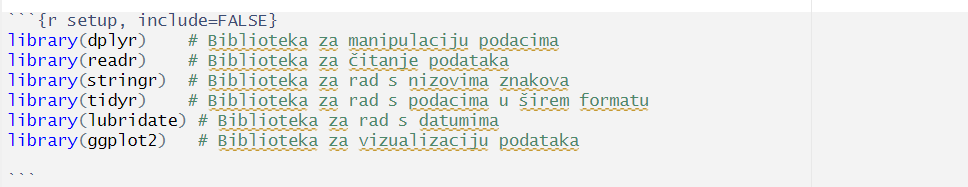
\includegraphics[scale=0.9]{slike/ucitavanje.png}
			% Veličina slike u odnosu na originalnu datoteku i pozicija slike
			\caption{\textbf{Učitavanje podataka u R-u}}
		\end{figure}
		
		U prikazanom kodu sa slike, koristimo različite R pakete kako bismo pripremili i istražili skup podataka "spotify\_songs.csv". Prvo, koristimo pakete poput \textbf{readr}, \textbf{dplyr} i \textbf{stringr} za čitanje i manipulaciju podacima. Nakon toga, prikazujemo prvih nekoliko redova podataka pomoću funkcije \textbf{head} kako bismo dobili inicijalni uvid u strukturu podataka.
		
		Zatim, koristimo funkciju \textbf{glimpse} za detaljniji pregled strukture podataka, prikazujući informacije o varijablama, njihovim tipovima podataka i prvim redovima podataka. Na kraju, koristimo funkciju \textbf{summary} kako bismo dobili osnovne statističke informacije o numeričkim varijablama u skupu podataka.
		
		Ovi koraci omogućuju nam osnovni uvid u strukturu podataka prije nego što nastavimo s daljnjom analizom i vizualizacijom.

	
	\subsubsection{Proces prilagodbe podataka}
	



\section{Vizualizacija Podataka}
	Vizualizacija podataka postaje ključna komponenta analize i interpretacije kompleksnih skupova podataka. 
	U ovom podpoglavlju istražujemo moć vizualizacije u kontekstu glazbene platforme Spotify, prezentirajući neke od grafova kako bismo bolje razumjeli glazbene obrasce, preferencije slušatelja te dinamiku glazbene industrije.
	
	\subsubsection{1) Histogram of song popularity}
	
	\textbf{Opis grafa:}
	
	Ovaj graf prikazuje histogram popularnosti. Prikazuje distribuciju popularnosti pjesama. Na x-osi nalaze se razine popularnosti pjesama, a y-osi broj pjesama koje se nalaze u pojedinoj razini popularnosti.
	Ovaj histogram omogućava vizualni pregled koje su razine popularnosti češće, a koje rjeđe. 

	\textbf{Slika grafa:}
	\begin{figure}[H]
		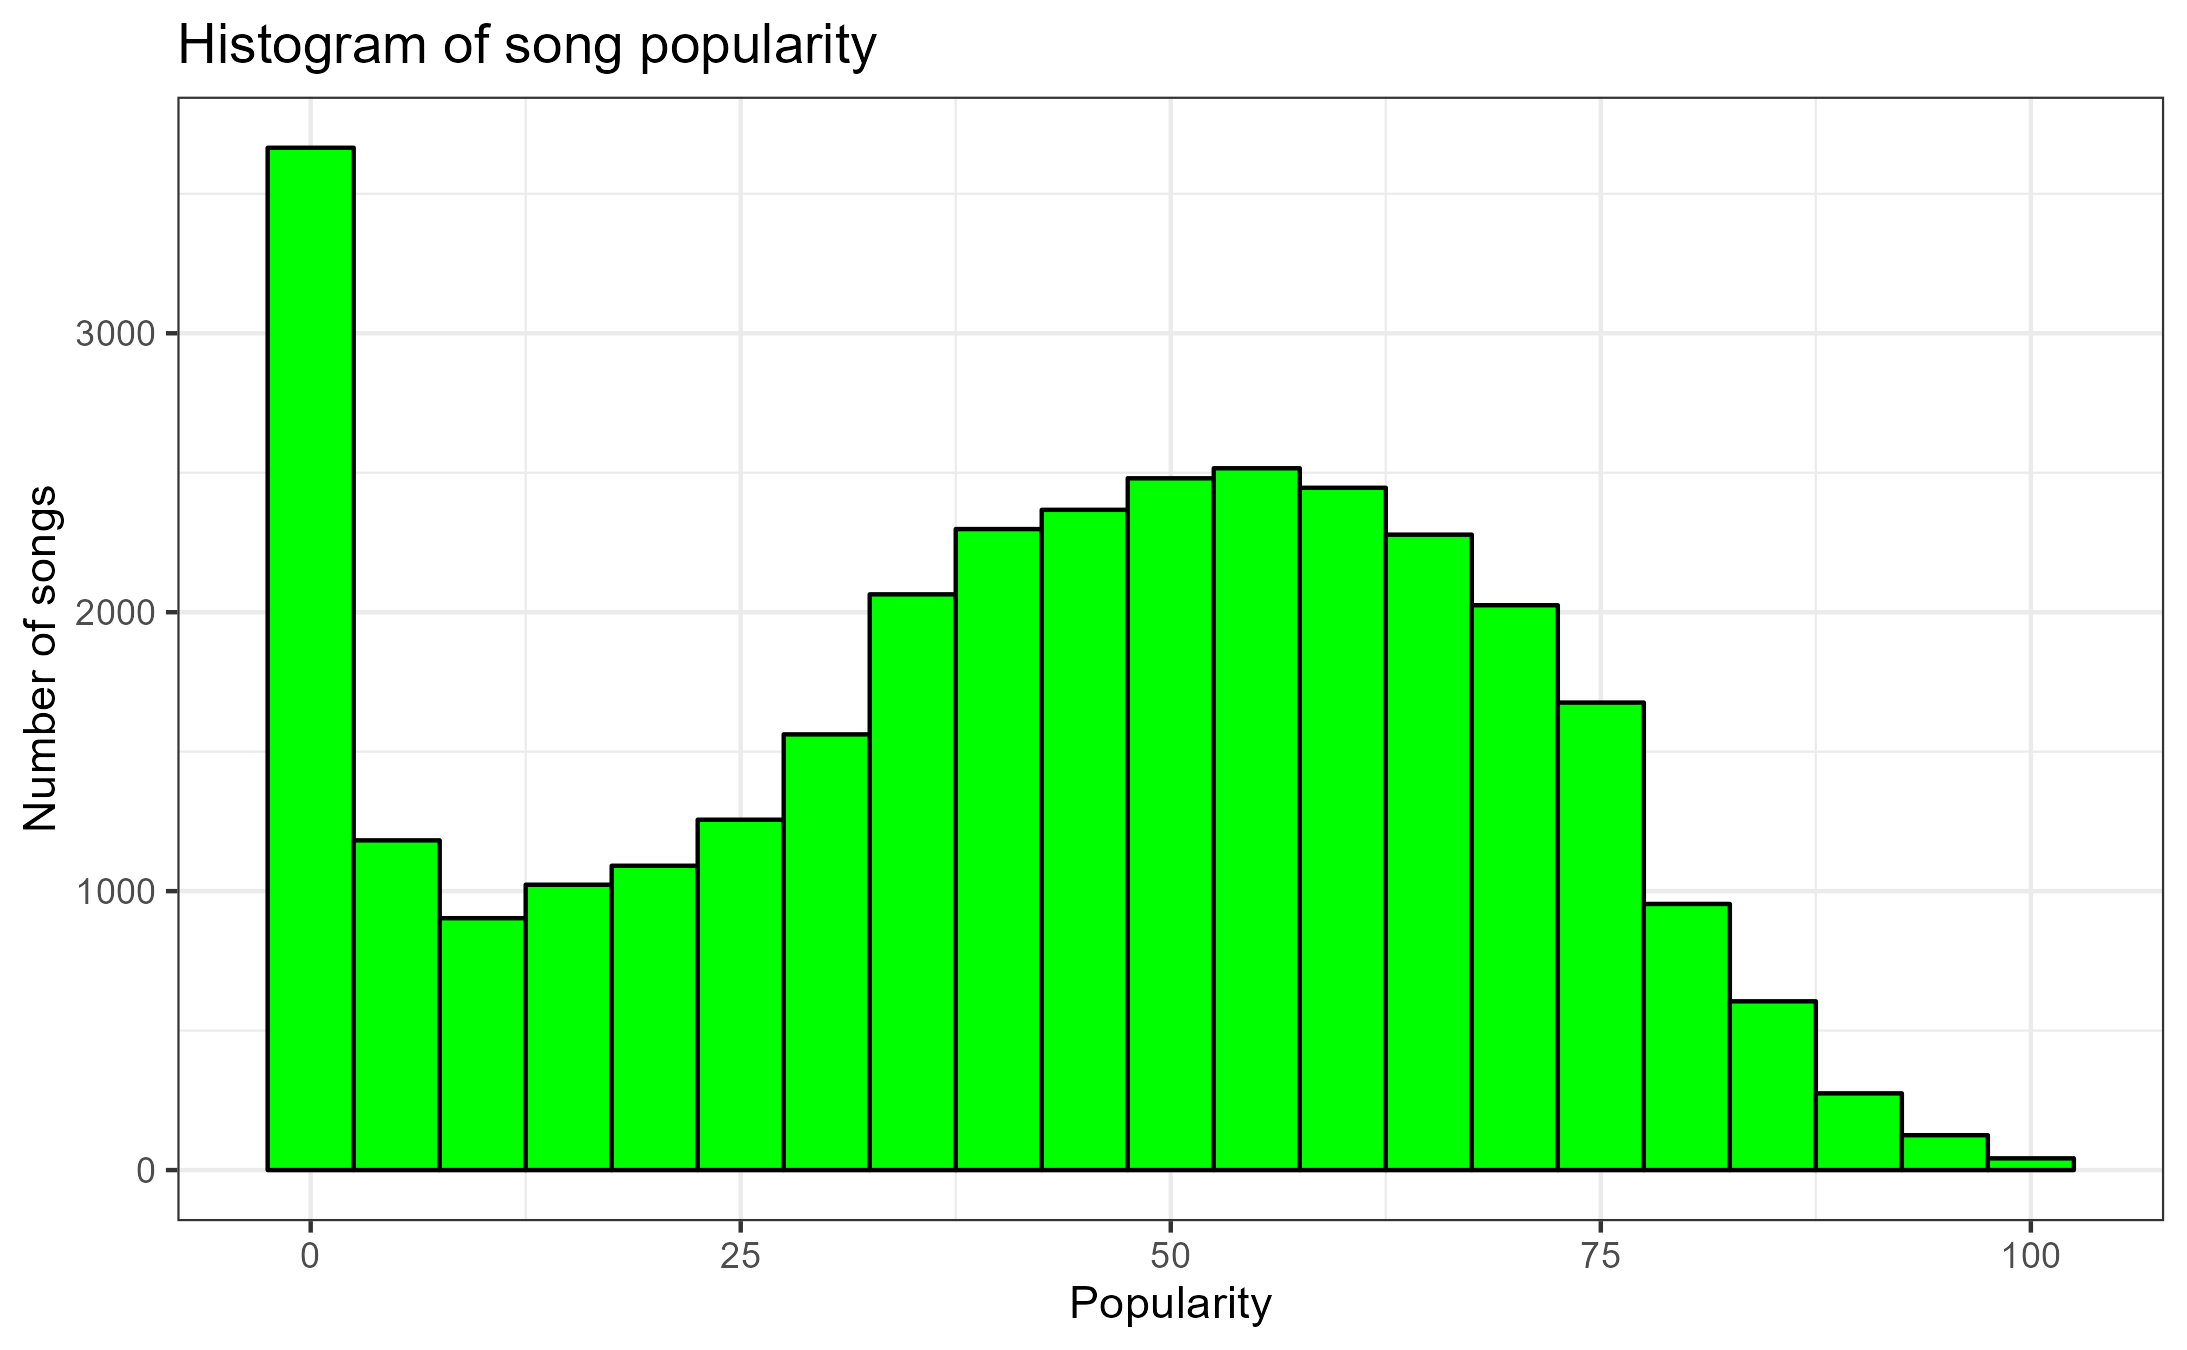
\includegraphics[scale=0.9]{slike/Histogram of song popularity.png}
		%veličina slike u odnosu na originalnu datoteku i pozicija slike
		\centering
		\caption{Histogram of song popularity}
		
	\end{figure}

	\subsubsection{2) Top 10 Artists Based on Popularity}
	
	\textbf{Opis grafa:}
	
	Ovaj graf prikazuje deset najpopularnijih glazbenih izvođača temeljem prosječne popularnosti njihovih pjesama. Izračunata je srednja vrijednost popularnosti za svakog izvođača, a zatim su odabrani najbolji deset izvođača prema toj mjeri popularnosti.
	
	Na x-osi su navedeni izvođači, poredani prema visini prosječne popularnosti, dok y-os prikazuje prosječnu popularnost. Svaki šareni stupac predstavlja jednog izvođača, a visina stupa označava njegovu prosječnu popularnost.
	
	Ovaj graf pruža brz i pregledan način usporedbe popularnosti izvođača, omogućujući identifikaciju najboljih deset temeljem prosjeka popularnosti njihovih pjesama.
	
	\textbf{Slika grafa:}
	\begin{figure}[H]
		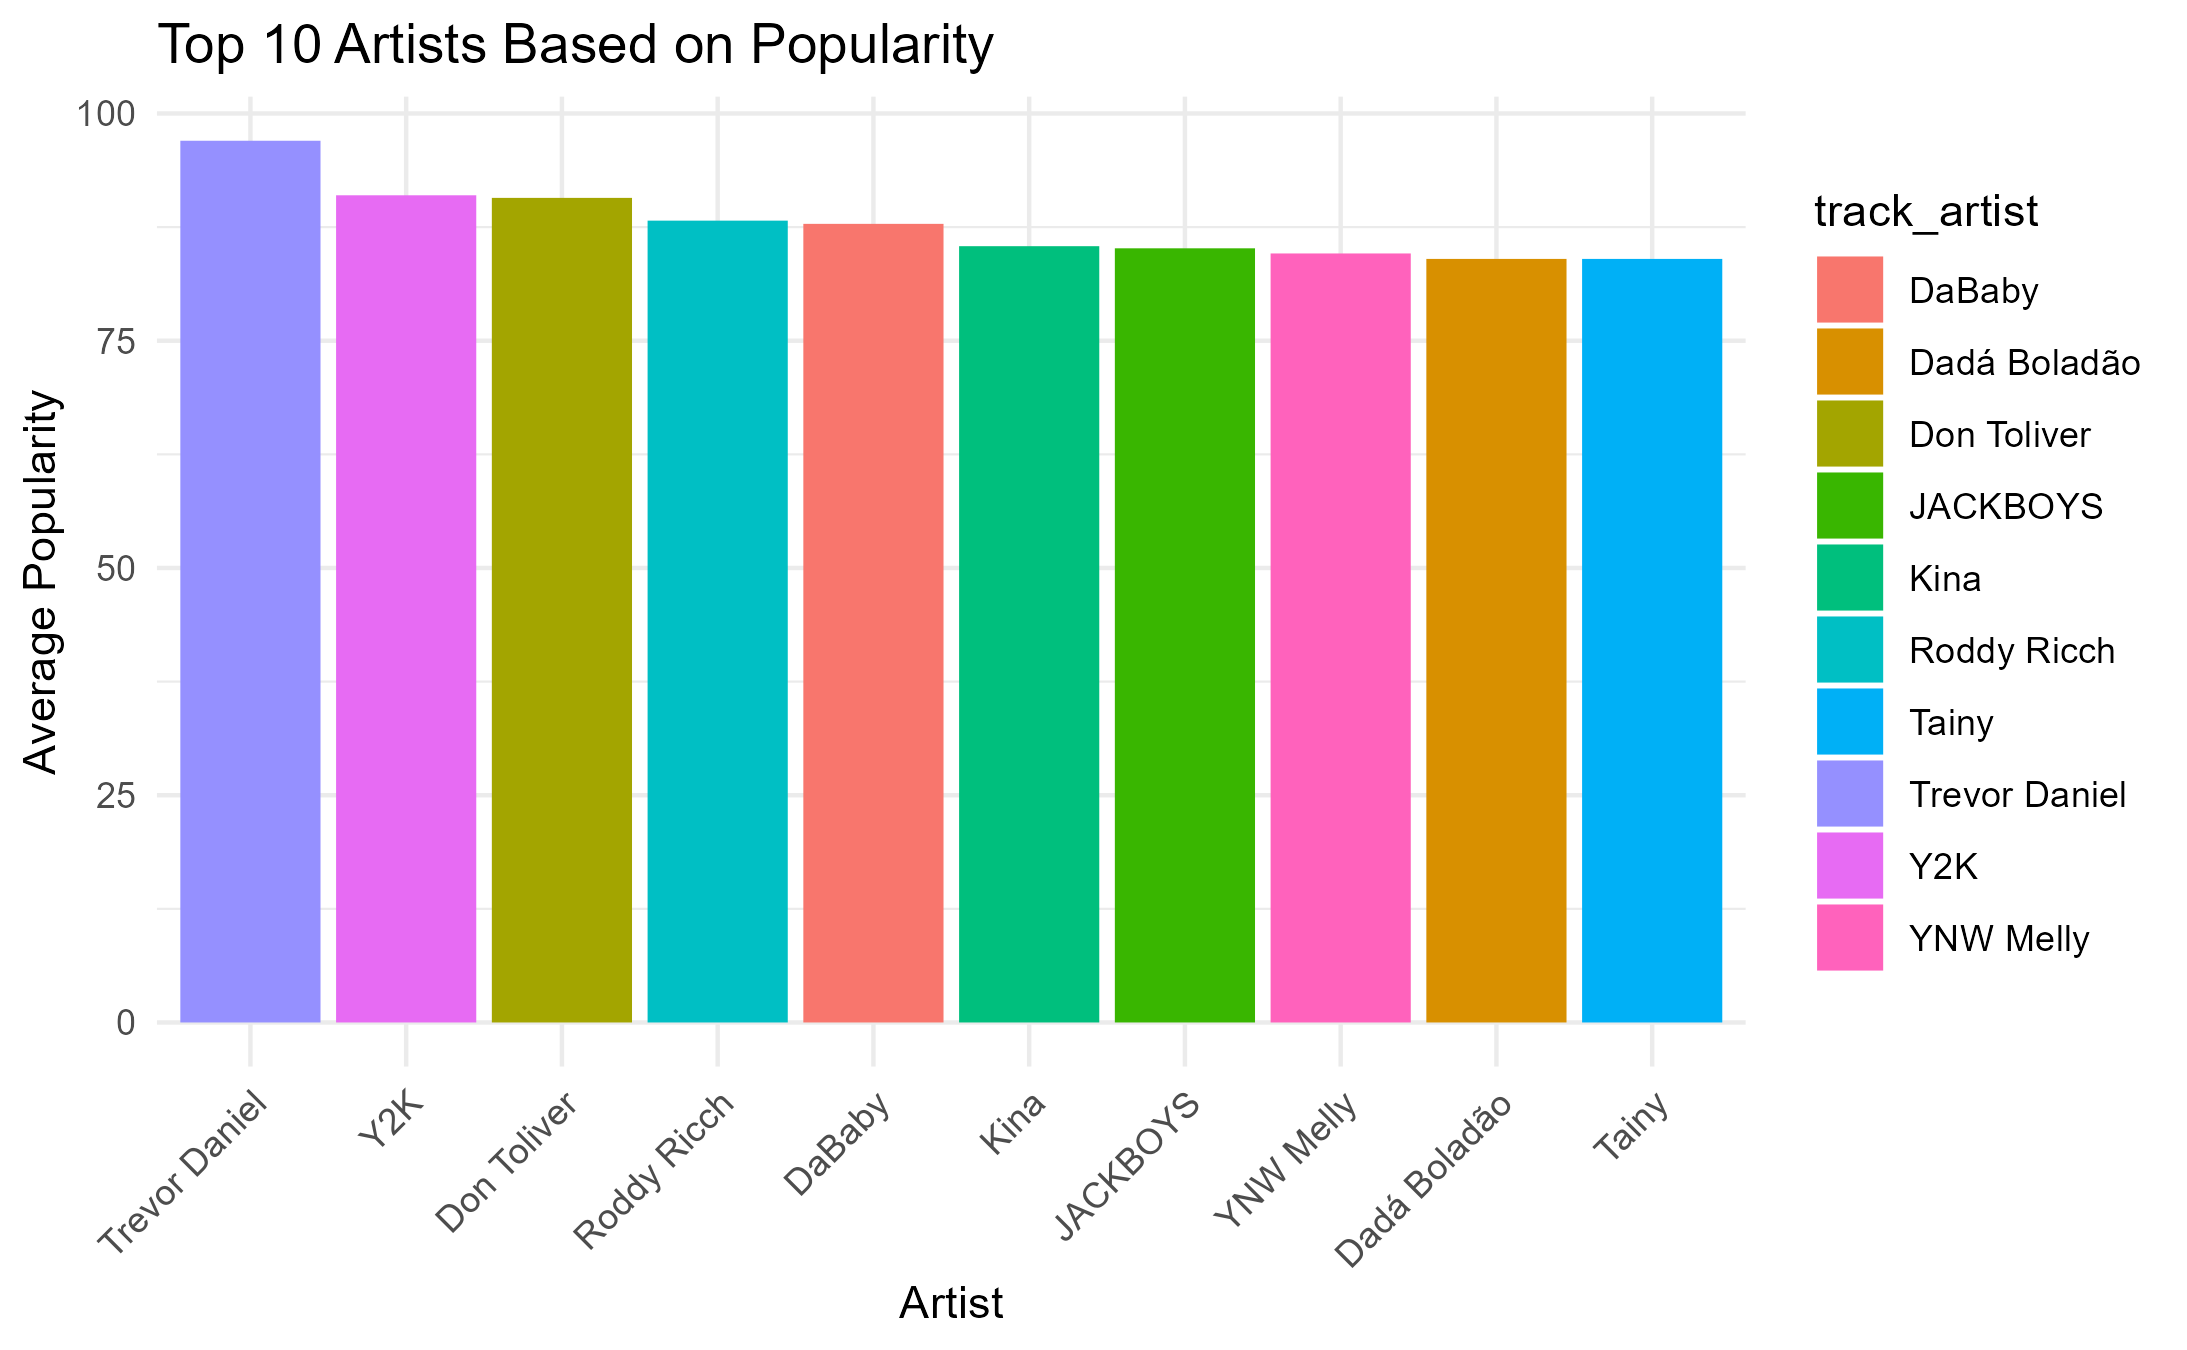
\includegraphics[scale=0.9]{slike/Top 10 popularity}
		%veličina slike u odnosu na originalnu datoteku i pozicija slike
		\centering
		\caption{Top 10 Artists Based on Popularity}
		
	\end{figure}


	\subsubsection{3) Average popularity of songs per year}
	
	\textbf{Opis grafa:}
	
	Ovaj stupčasti graf prikazuje prosječnu popularnost pjesama po godinama u razdoblju od 2000. godine do 2020. godine. X-os ovog grafa su godine u navedenom razdoblju (svaki stupac predstavlja jednu godinu), dok y-os predstavlja prosječnu popularnost. 
	Uvidom u ovaj graf možemo jednostavno vidjeti u kojoj su godini pjesme imale najveću popularnost, te vidjeti kako se popularnost mijenjala tokom tih 20 godina.

	
	\textbf{Slika grafa:}
	\begin{figure}[H]
		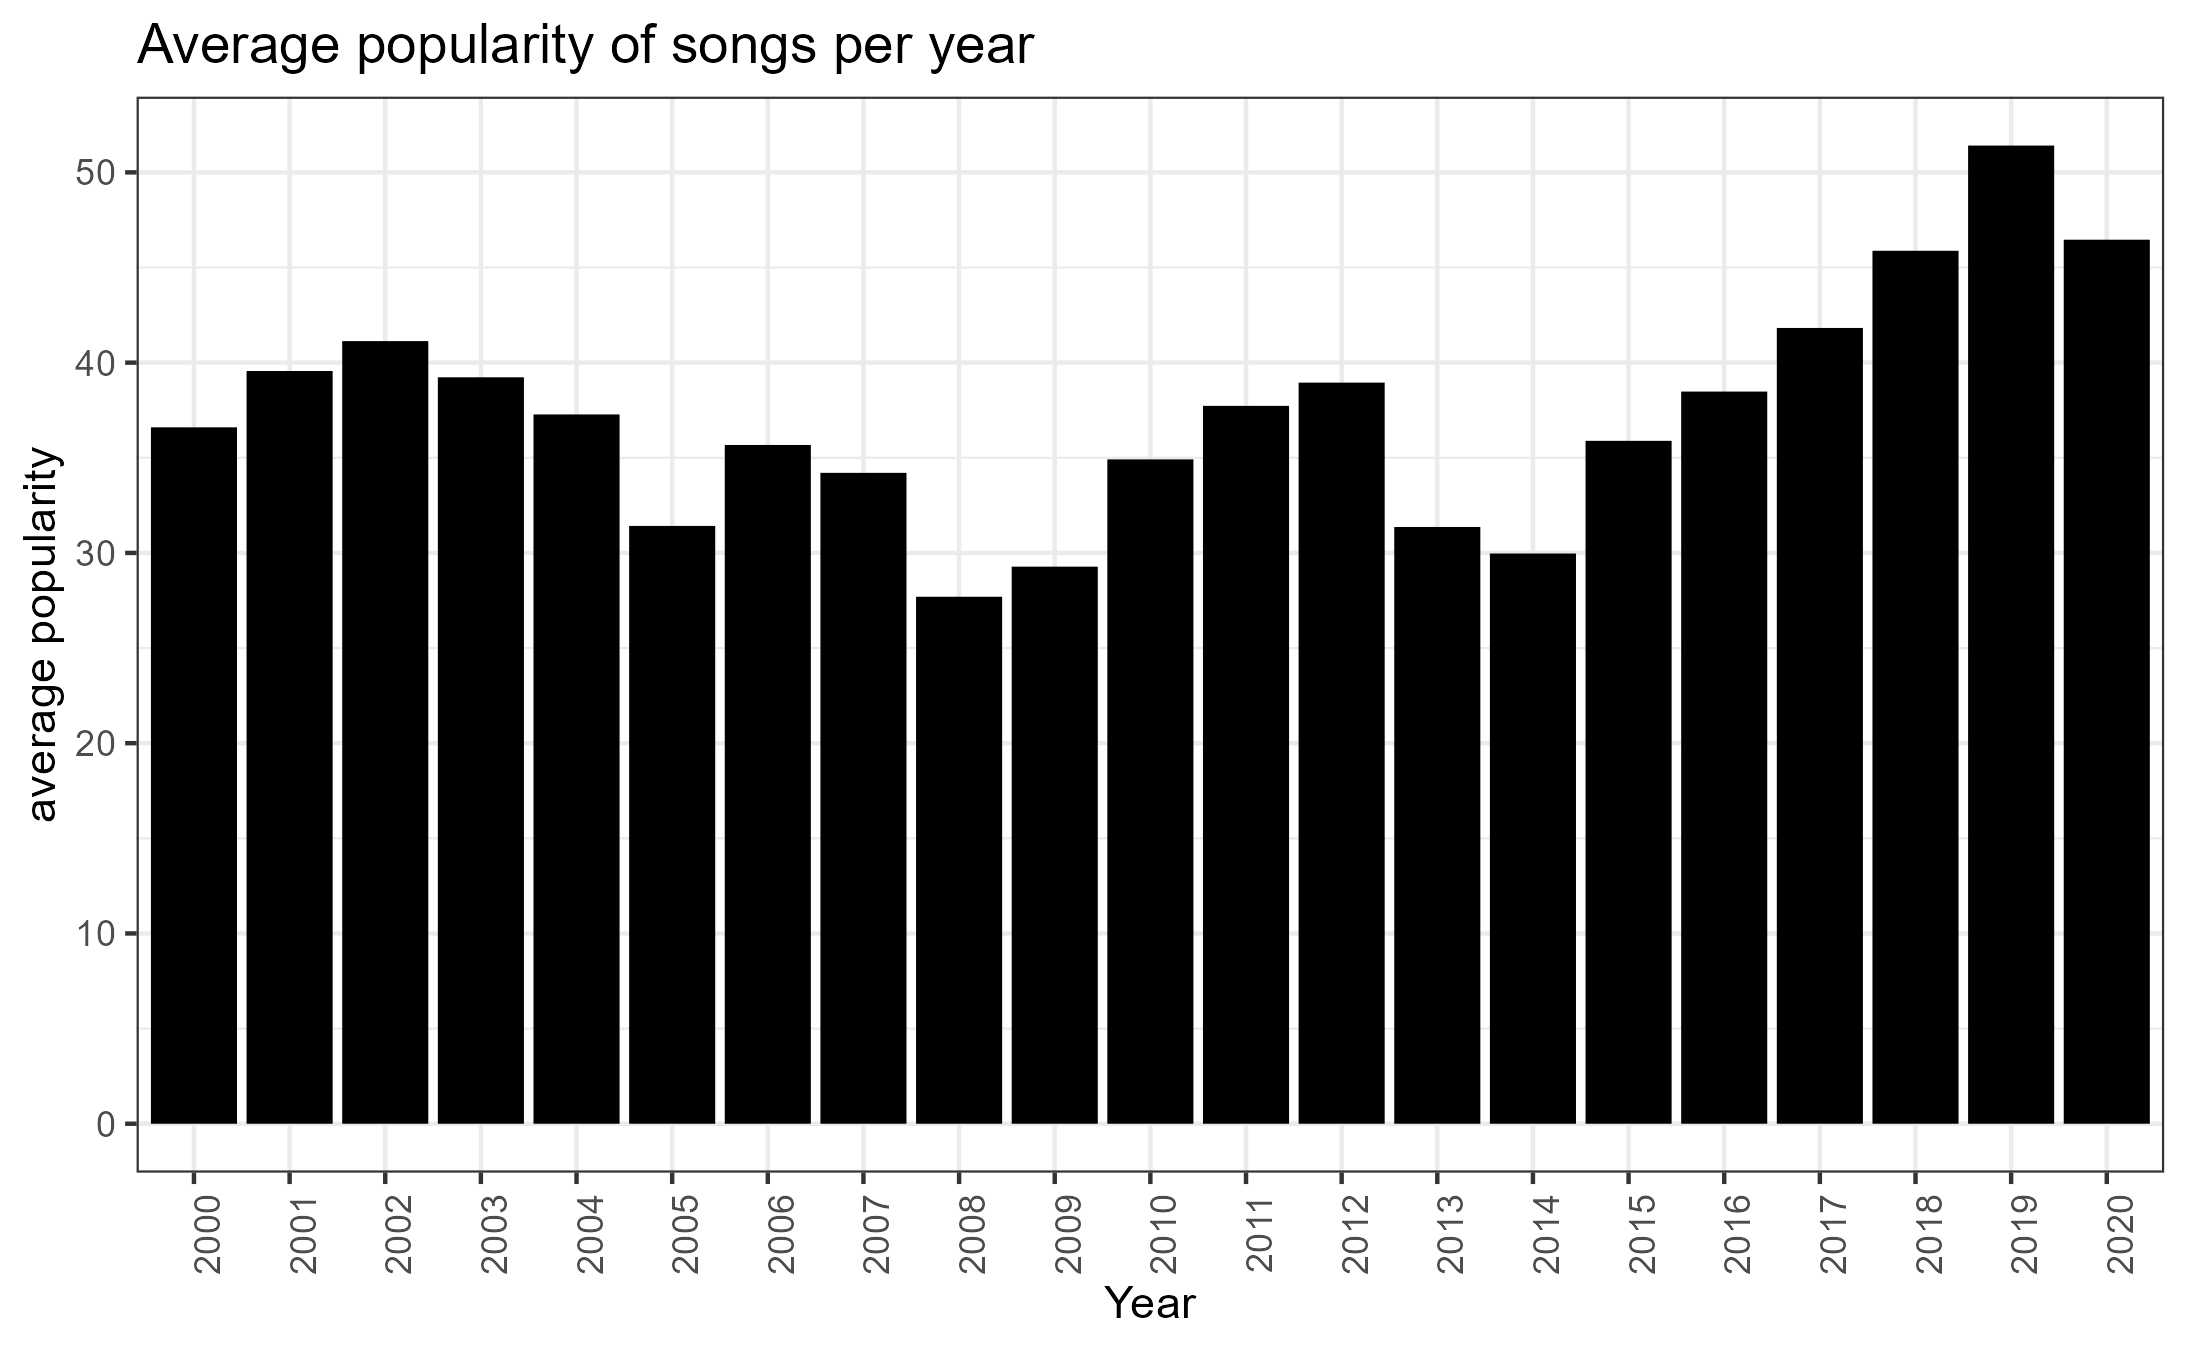
\includegraphics[scale=0.9]{slike/Average popularity of songs per year.png}
		%veličina slike u odnosu na originalnu datoteku i pozicija slike
		\centering
		\caption{Average popularity of songs per year}
		
	\end{figure}
	
		\subsubsection{4) Energy Distribution Across Playlist Genre}
	
	\textbf{Opis grafa:}
	
	Ovaj graf prikazuje distribuciju energije (y-os) na temelju različitih žanrova playlista (x-os). Svaki boxplot predstavlja jedan žanr, a njegova visina odražava raspon energije unutar tog žanra. Unutar svakog boxplota nalazi se pravokutnik koji predstavlja interkvartilni raspon, a linija unutar pravokutnika označava medijan energije.
	
	Dodatno, postojanje "notcha" u sredini svakog boxplota pruža informaciju o razlikama u medijanima između žanrova.
	
	
	\textbf{Slika grafa:}
	\begin{figure}[H]
		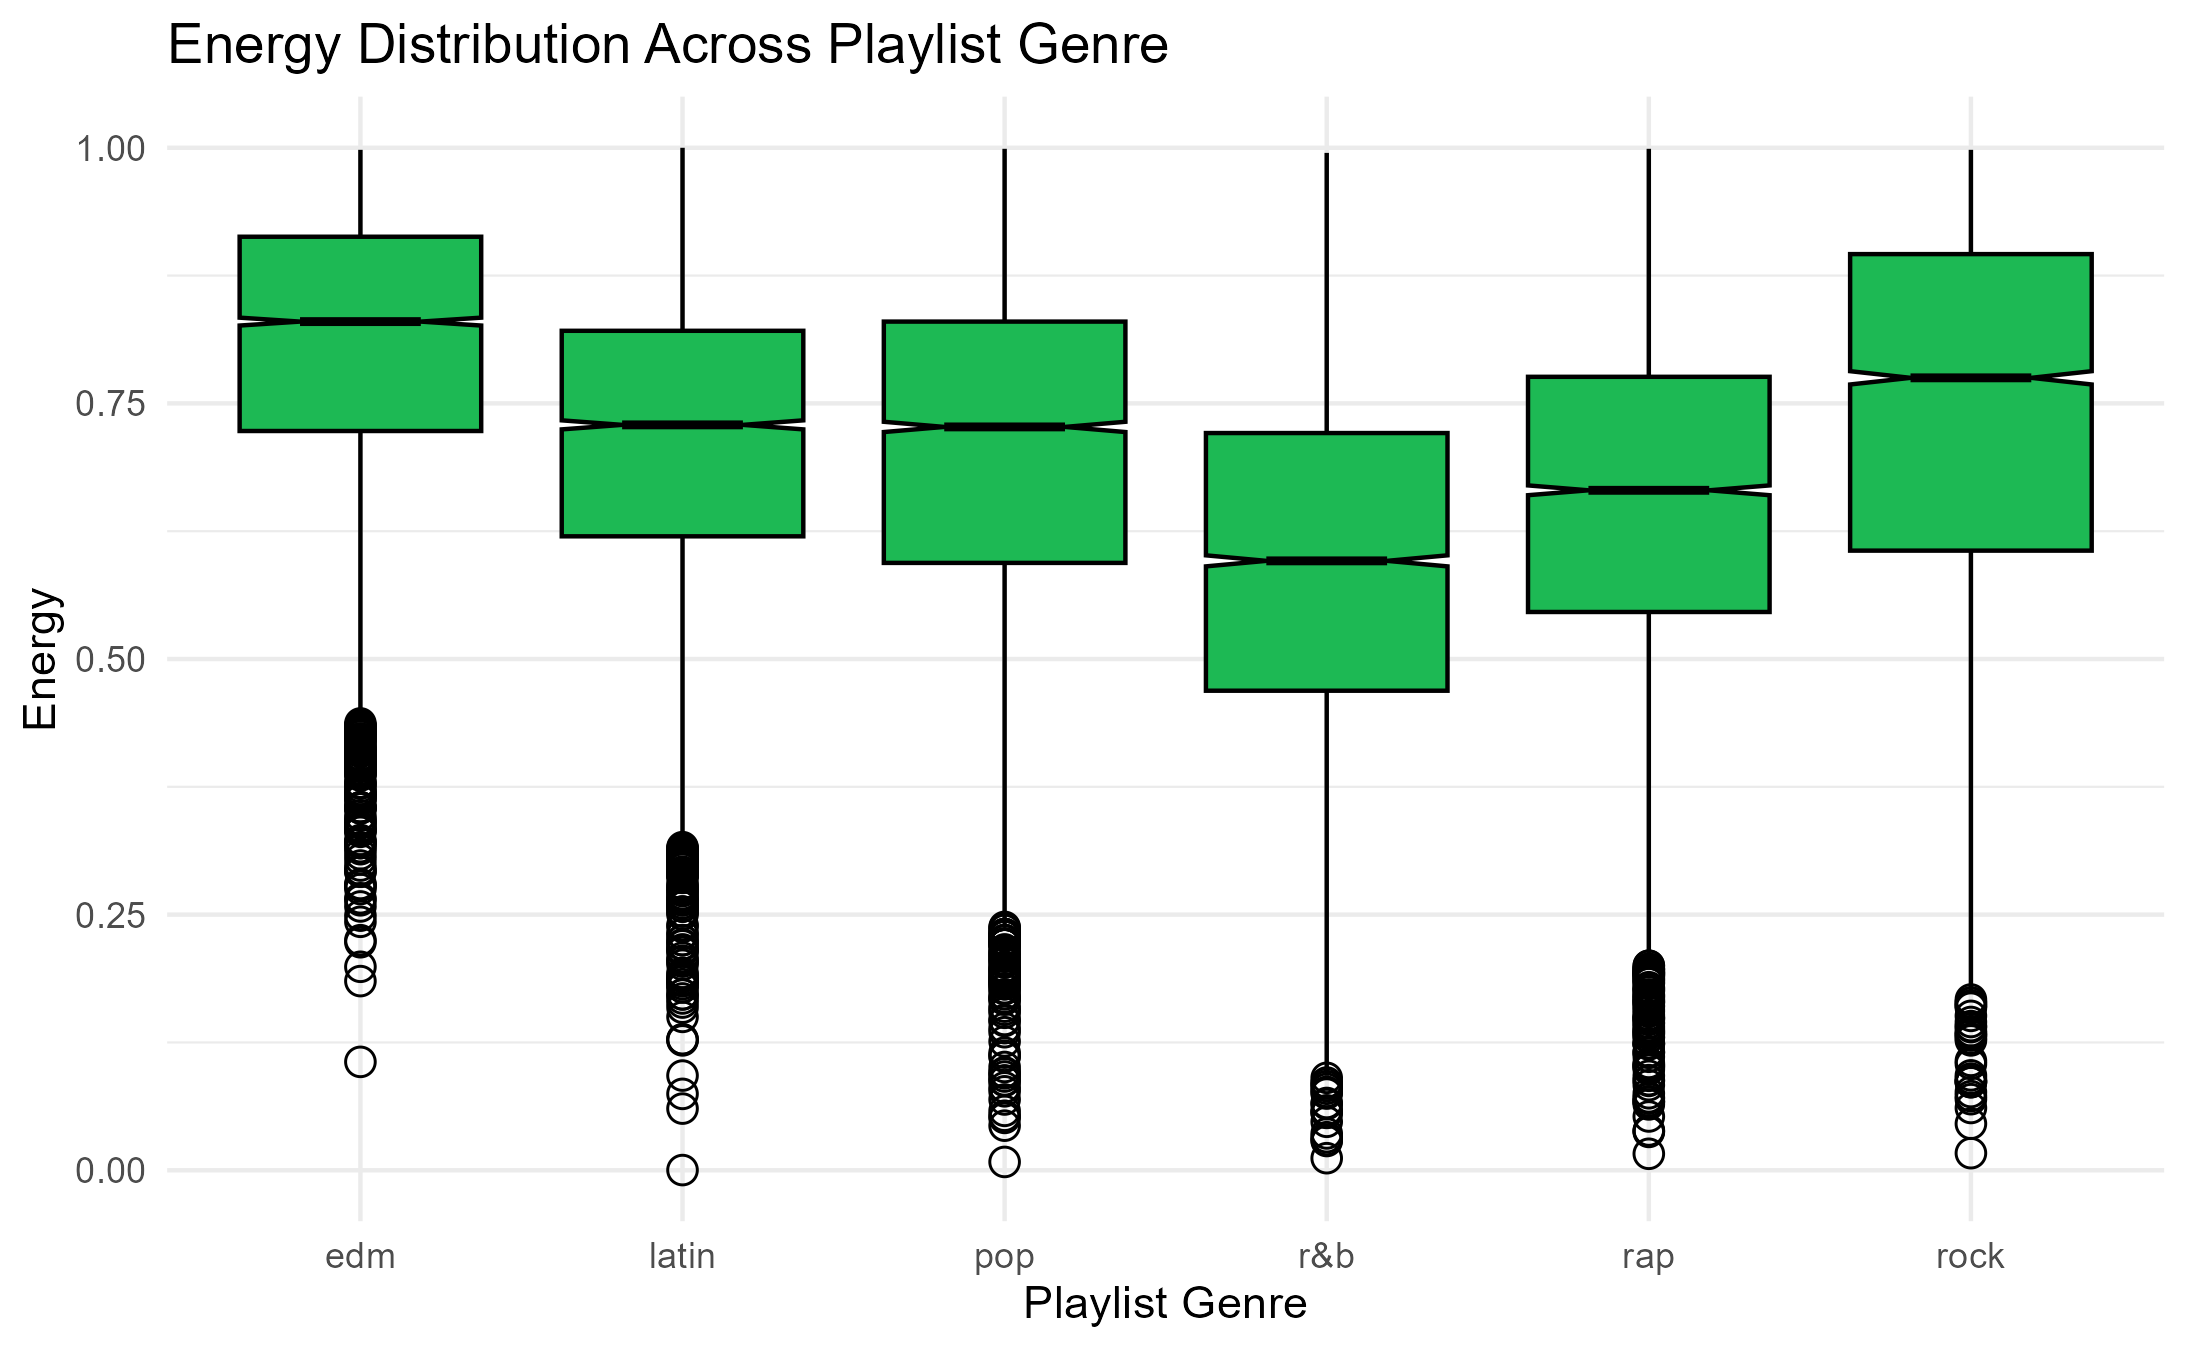
\includegraphics[scale=0.9]{slike/Genre-Energy.png}
		%veličina slike u odnosu na originalnu datoteku i pozicija slike
		\centering
		\caption{Energy Distribution Across Playlist Genre}
		
	\end{figure}
	
		\subsubsection{5) Distribution of Genres and Subgenres}
	
	\textbf{Opis grafa:}
	
		Ovaj graf prikazuje broj playlista unutar određenih glavnih žanrova, razdijeljenih prema podžanrovima. Na x-osi su navedeni glavni žanrovi playlista, dok y-os pokazuje broj playlista. Svaki šareni segment na stupcu predstavlja određeni podžanr unutar glavnog žanra.
		
		Stupci su složeni jedan na drugi kako bi se vizualno prikazala distribucija podžanrova u okviru svakog glavnog žanra. 
	
	
	\textbf{Slika grafa:}
	\begin{figure}[H]
		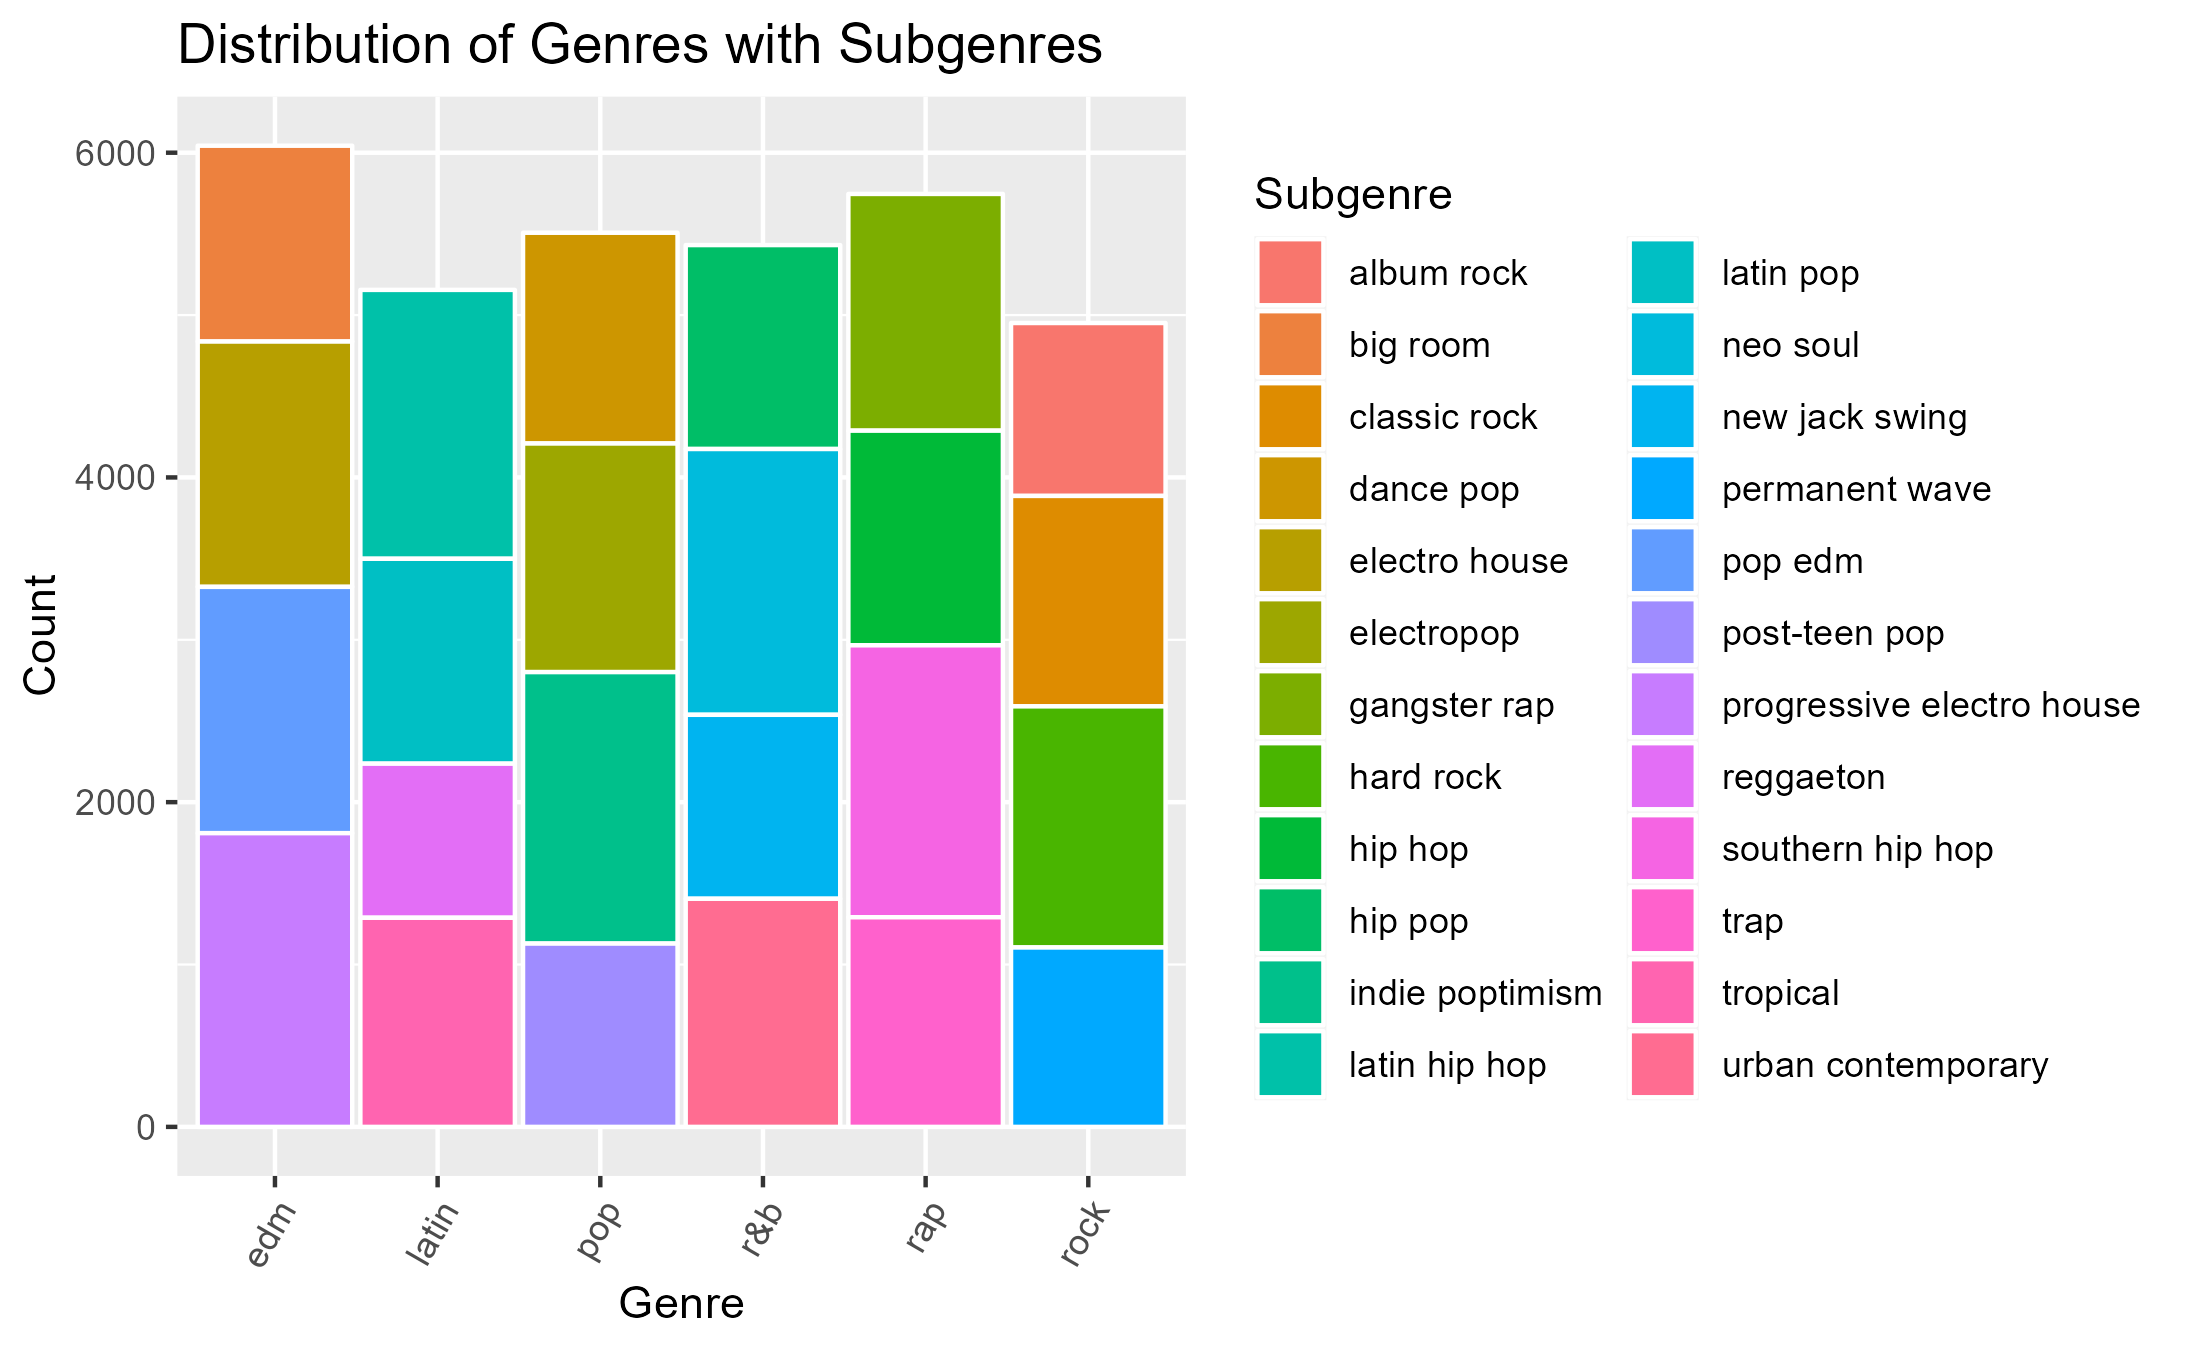
\includegraphics[scale=0.9]{slike/Genre-Subgenre.png}
		%veličina slike u odnosu na originalnu datoteku i pozicija slike
		\centering
		\caption{Distribution of Genres and Subgenres}
		
	\end{figure}


		\subsubsection{6) The relationship between energy and valence by genre}
    
    \textbf{Opis grafa:}
    
    	Ovaj graf prikazuje odnos između energije i valencije. N a x-osi nalazi se energija koja može biti u rasponu između 0 i 1, a na y-osi nalazi se valencija koja može biti u isto rasponu kao i energija. Svaka točka na grafu prikazuje jednu pjesmu , a njezina pozicija prikazuje odnos energija-valencija. Svaka boja točke prikazuje različiti žanr. 
    
    \textbf{Slika grafa:}
    \begin{figure}[H]
        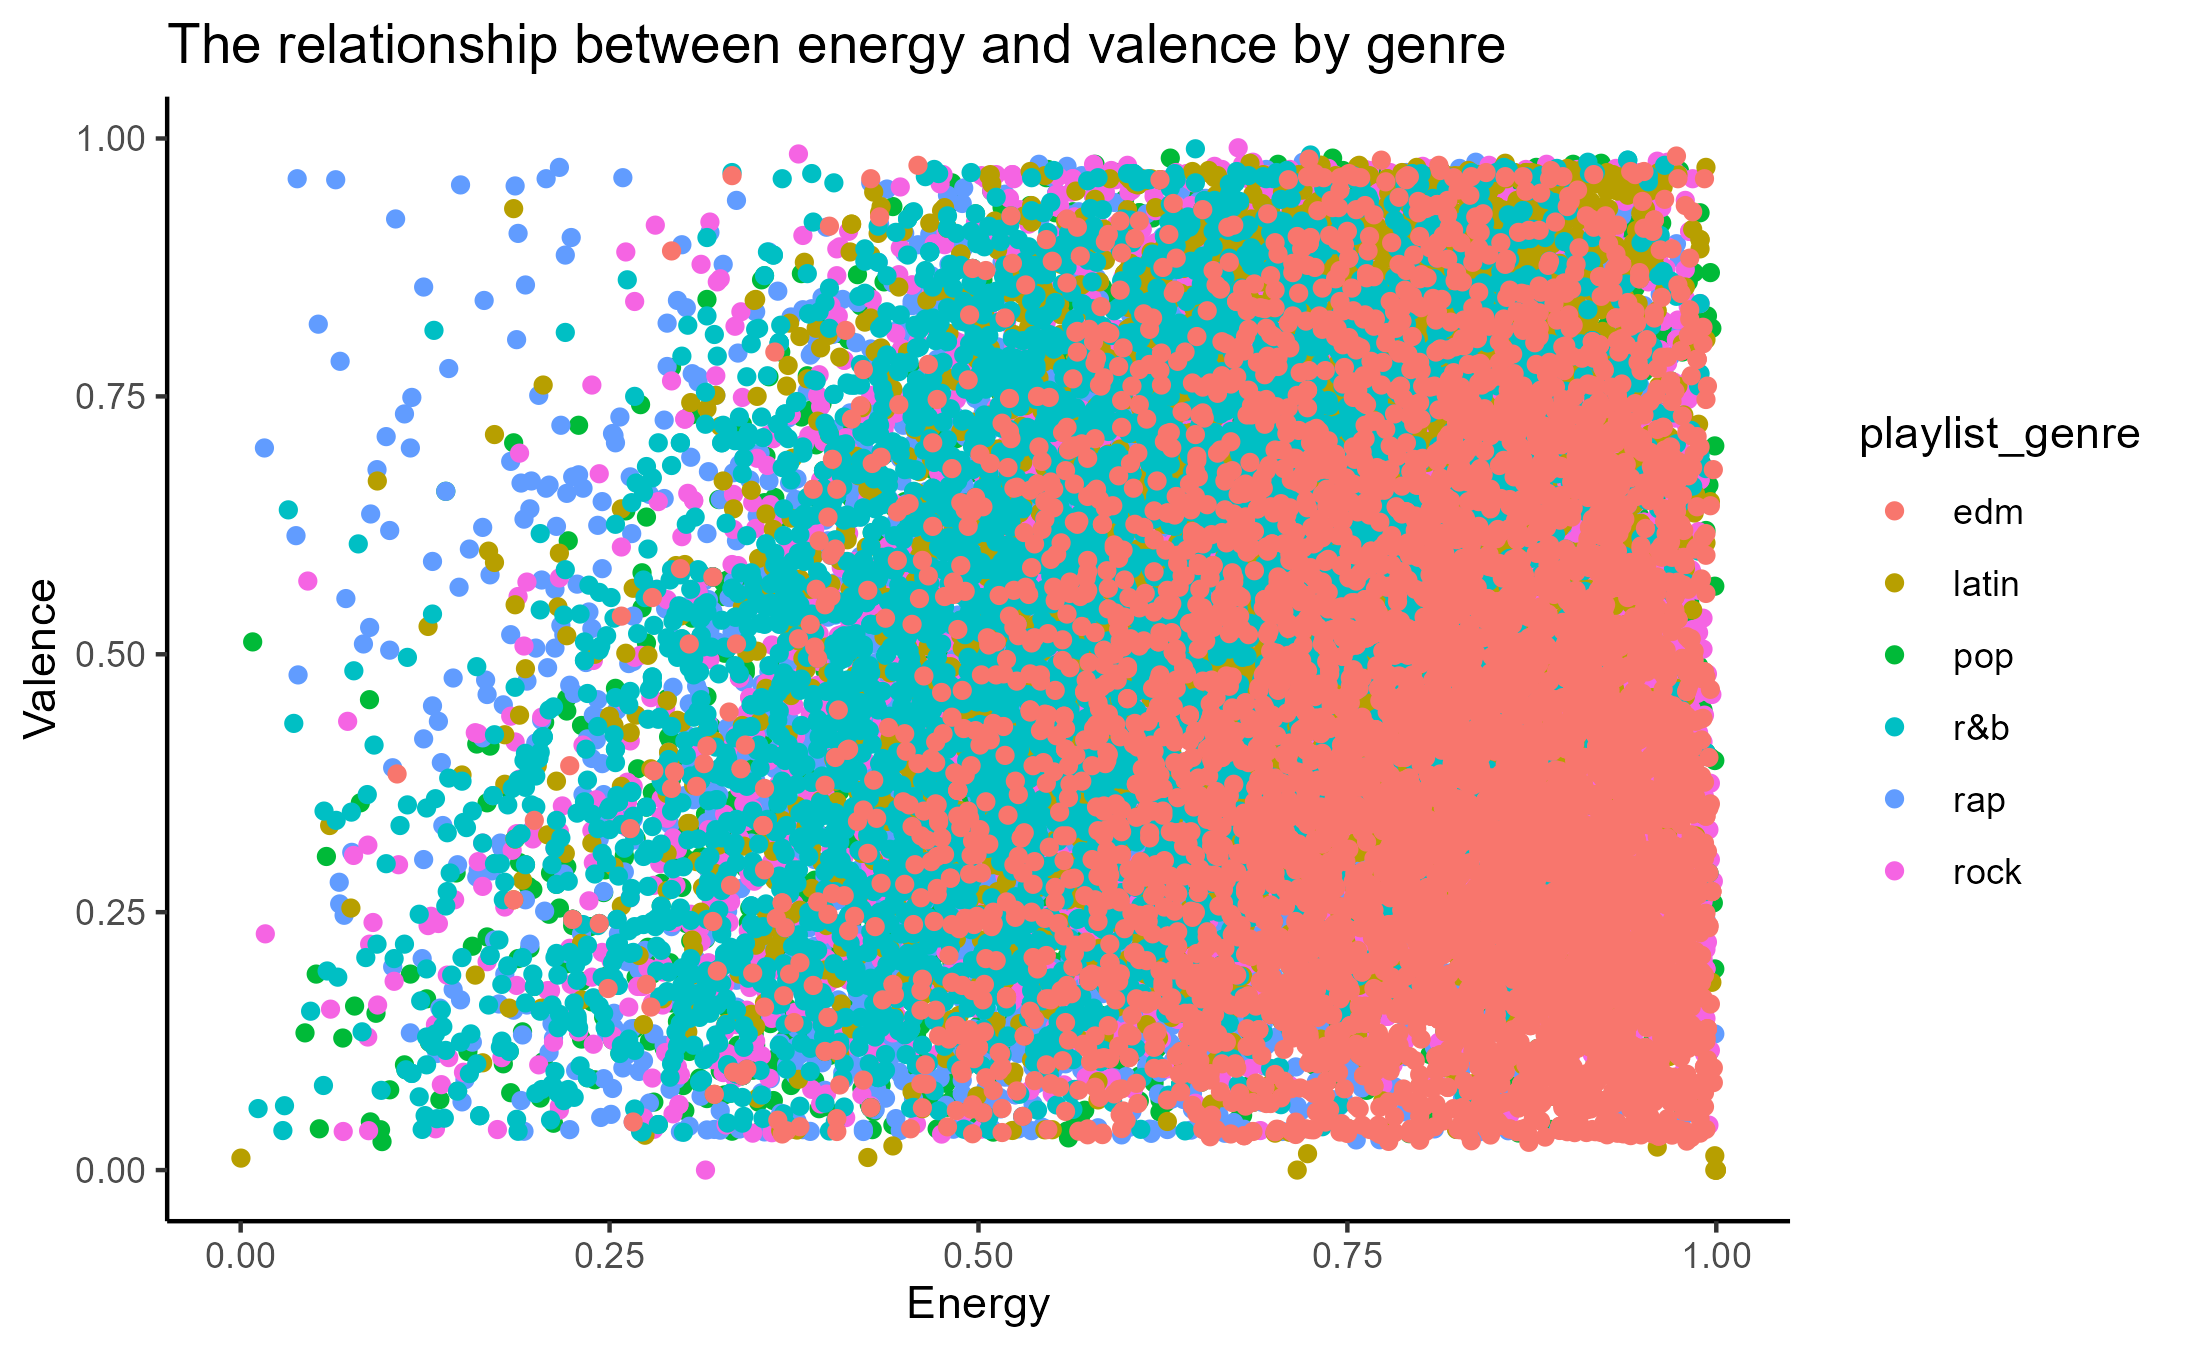
\includegraphics[scale=0.9]{slike/The relationship between energy and valence by genre.png}
        %veličina slike u odnosu na originalnu datoteku i pozicija slike
        \centering
        \caption{The relationship between energy ad valence by genre}
        
    \end{figure}

	
		\subsubsection{7) Danceability and Energy with Popularity}
	
	\textbf{Opis grafa:}
	
	Ovaj šareni graf prikazuje odnos između plesnosti (x-os) i energije (y-os) za različite glazbene pjesme. Svaka točka na grafu predstavlja pojedinu pjesmu, a njezina boja označava razinu popularnosti. Tamnije crvene nijanse označavaju popularnije pjesme, dok svjetlije plave nijanse ukazuju na manju popularnost.
	
	Graf pruža uvid u raznolikost glazbenih preferencija te naglašava da glazbene osobitosti kao što su plesnost i energija nisu nužno ključni faktori koji određuju popularnost pjesama na temelju analize ovog skupa podataka.
	
	\textbf{Slika grafa:}
	\begin{figure}[H]
		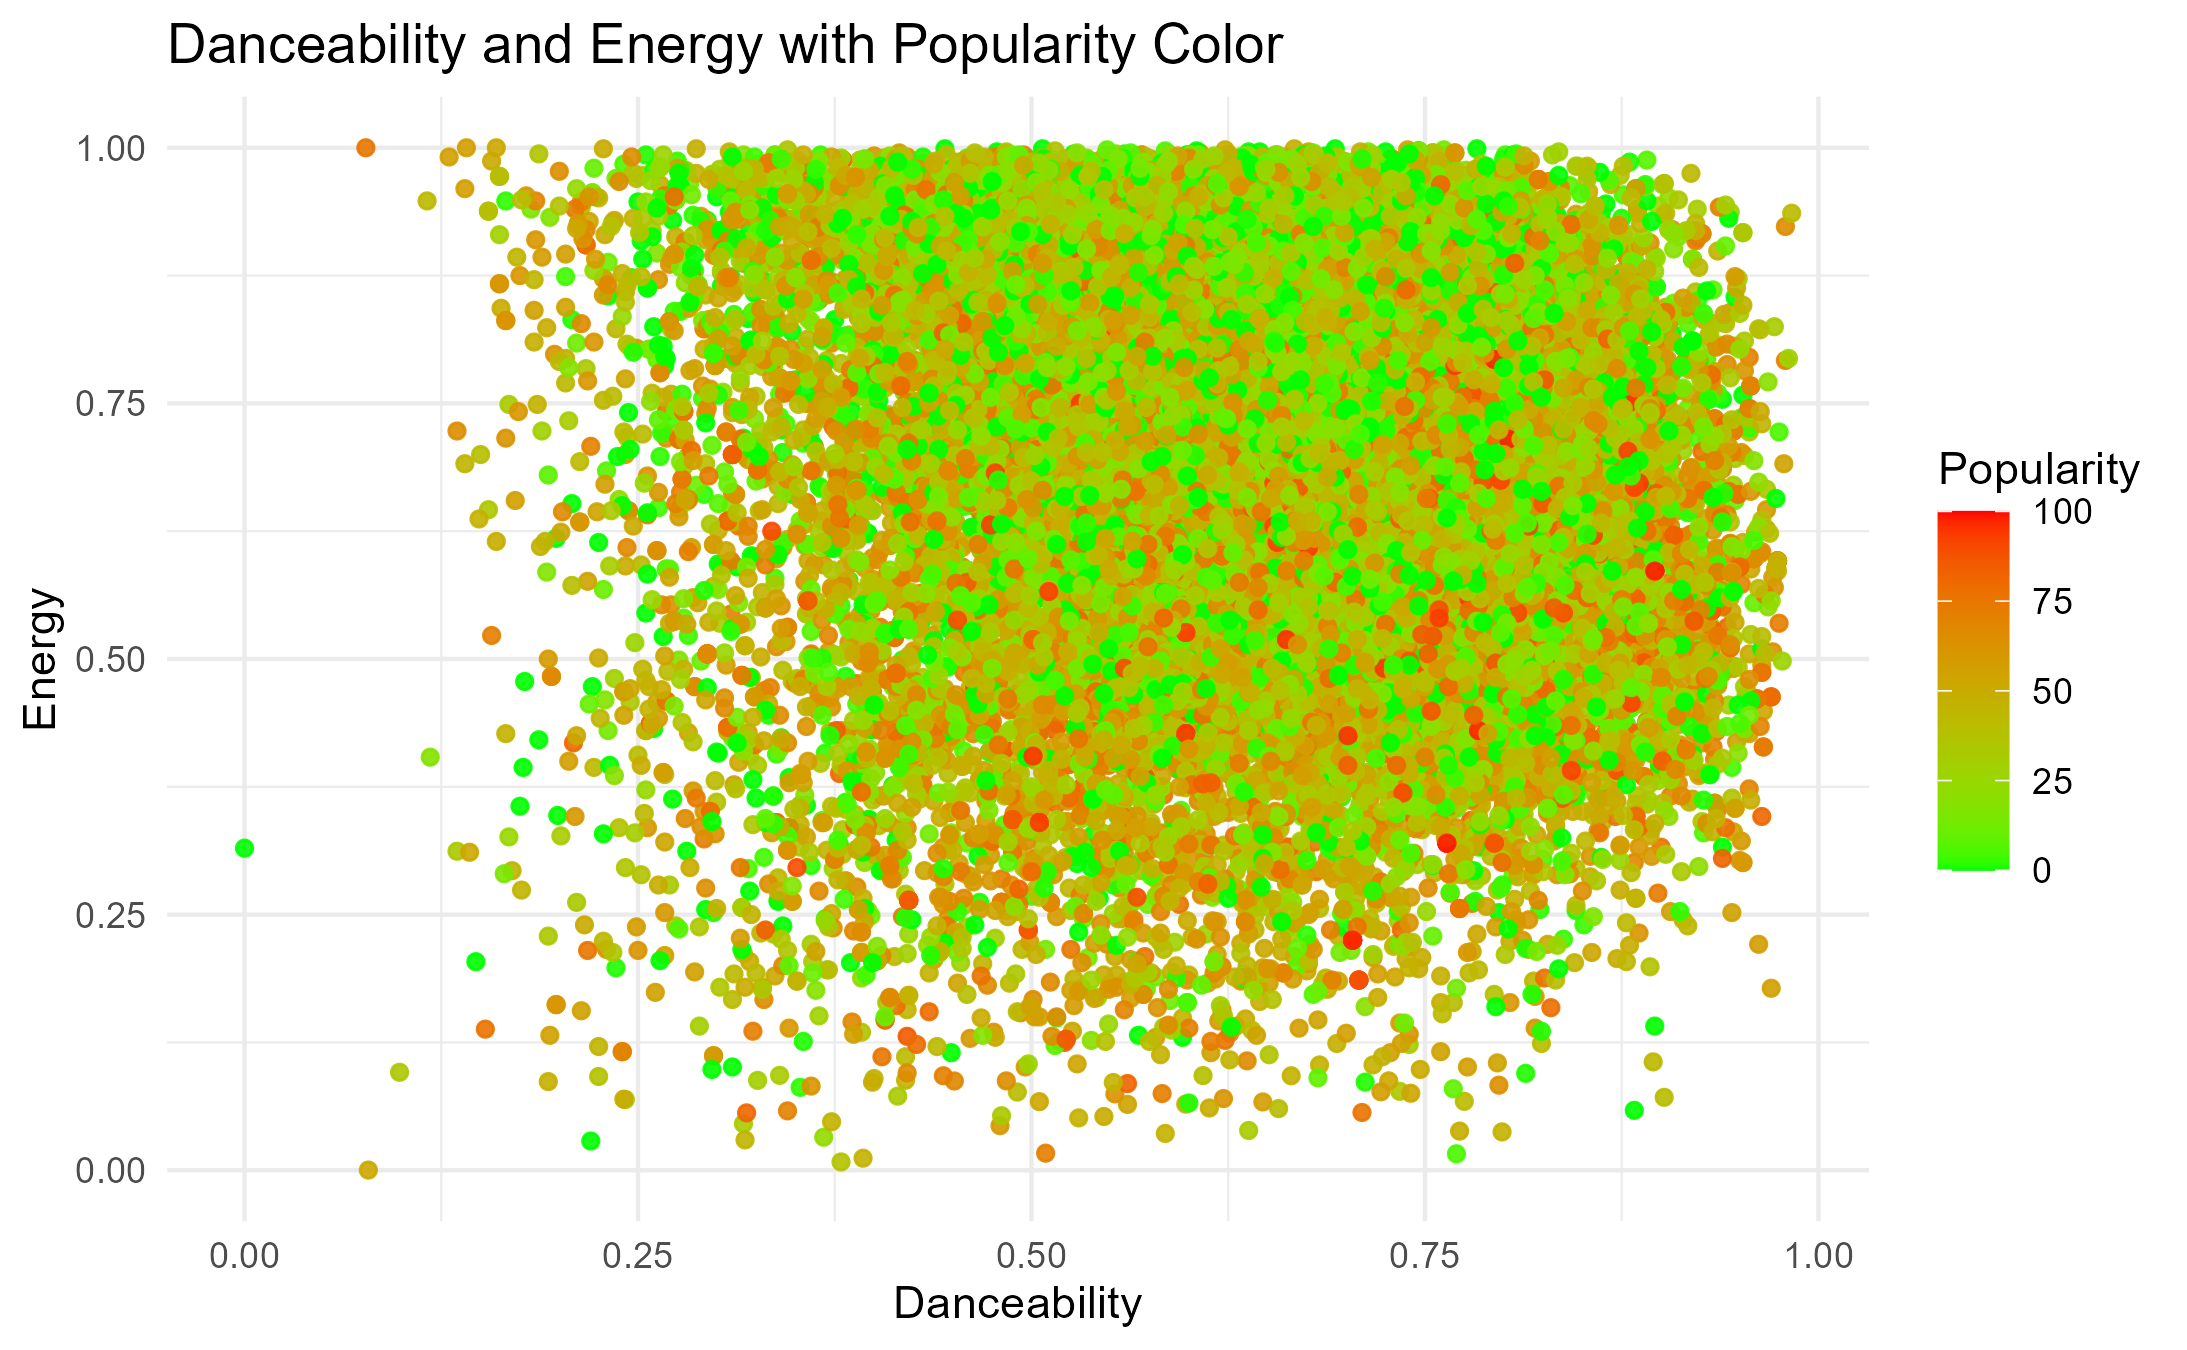
\includegraphics[scale=0.9]{slike/Dance-Energy-popularity.png}
		%veličina slike u odnosu na originalnu datoteku i pozicija slike
		\centering
		\caption{ Danceability and Energy with Popularity}
		
	\end{figure}


	\subsubsection{8) Histogram of song durations}
    
    \textbf{Opis grafa:}
    
Ovaj graf pruža uvid u distribuciju trajanja pjesama. Na x-osi nalaze se različite razine trajanju u sekundama, dok y-os predstavlja broj pjesma u pojedinoj razini. Ovaj zanimljiv histogram omogućava vizualni o najčešćem trajanju pjesama.
    

    \textbf{Slika grafa:}
    \begin{figure}[H]
        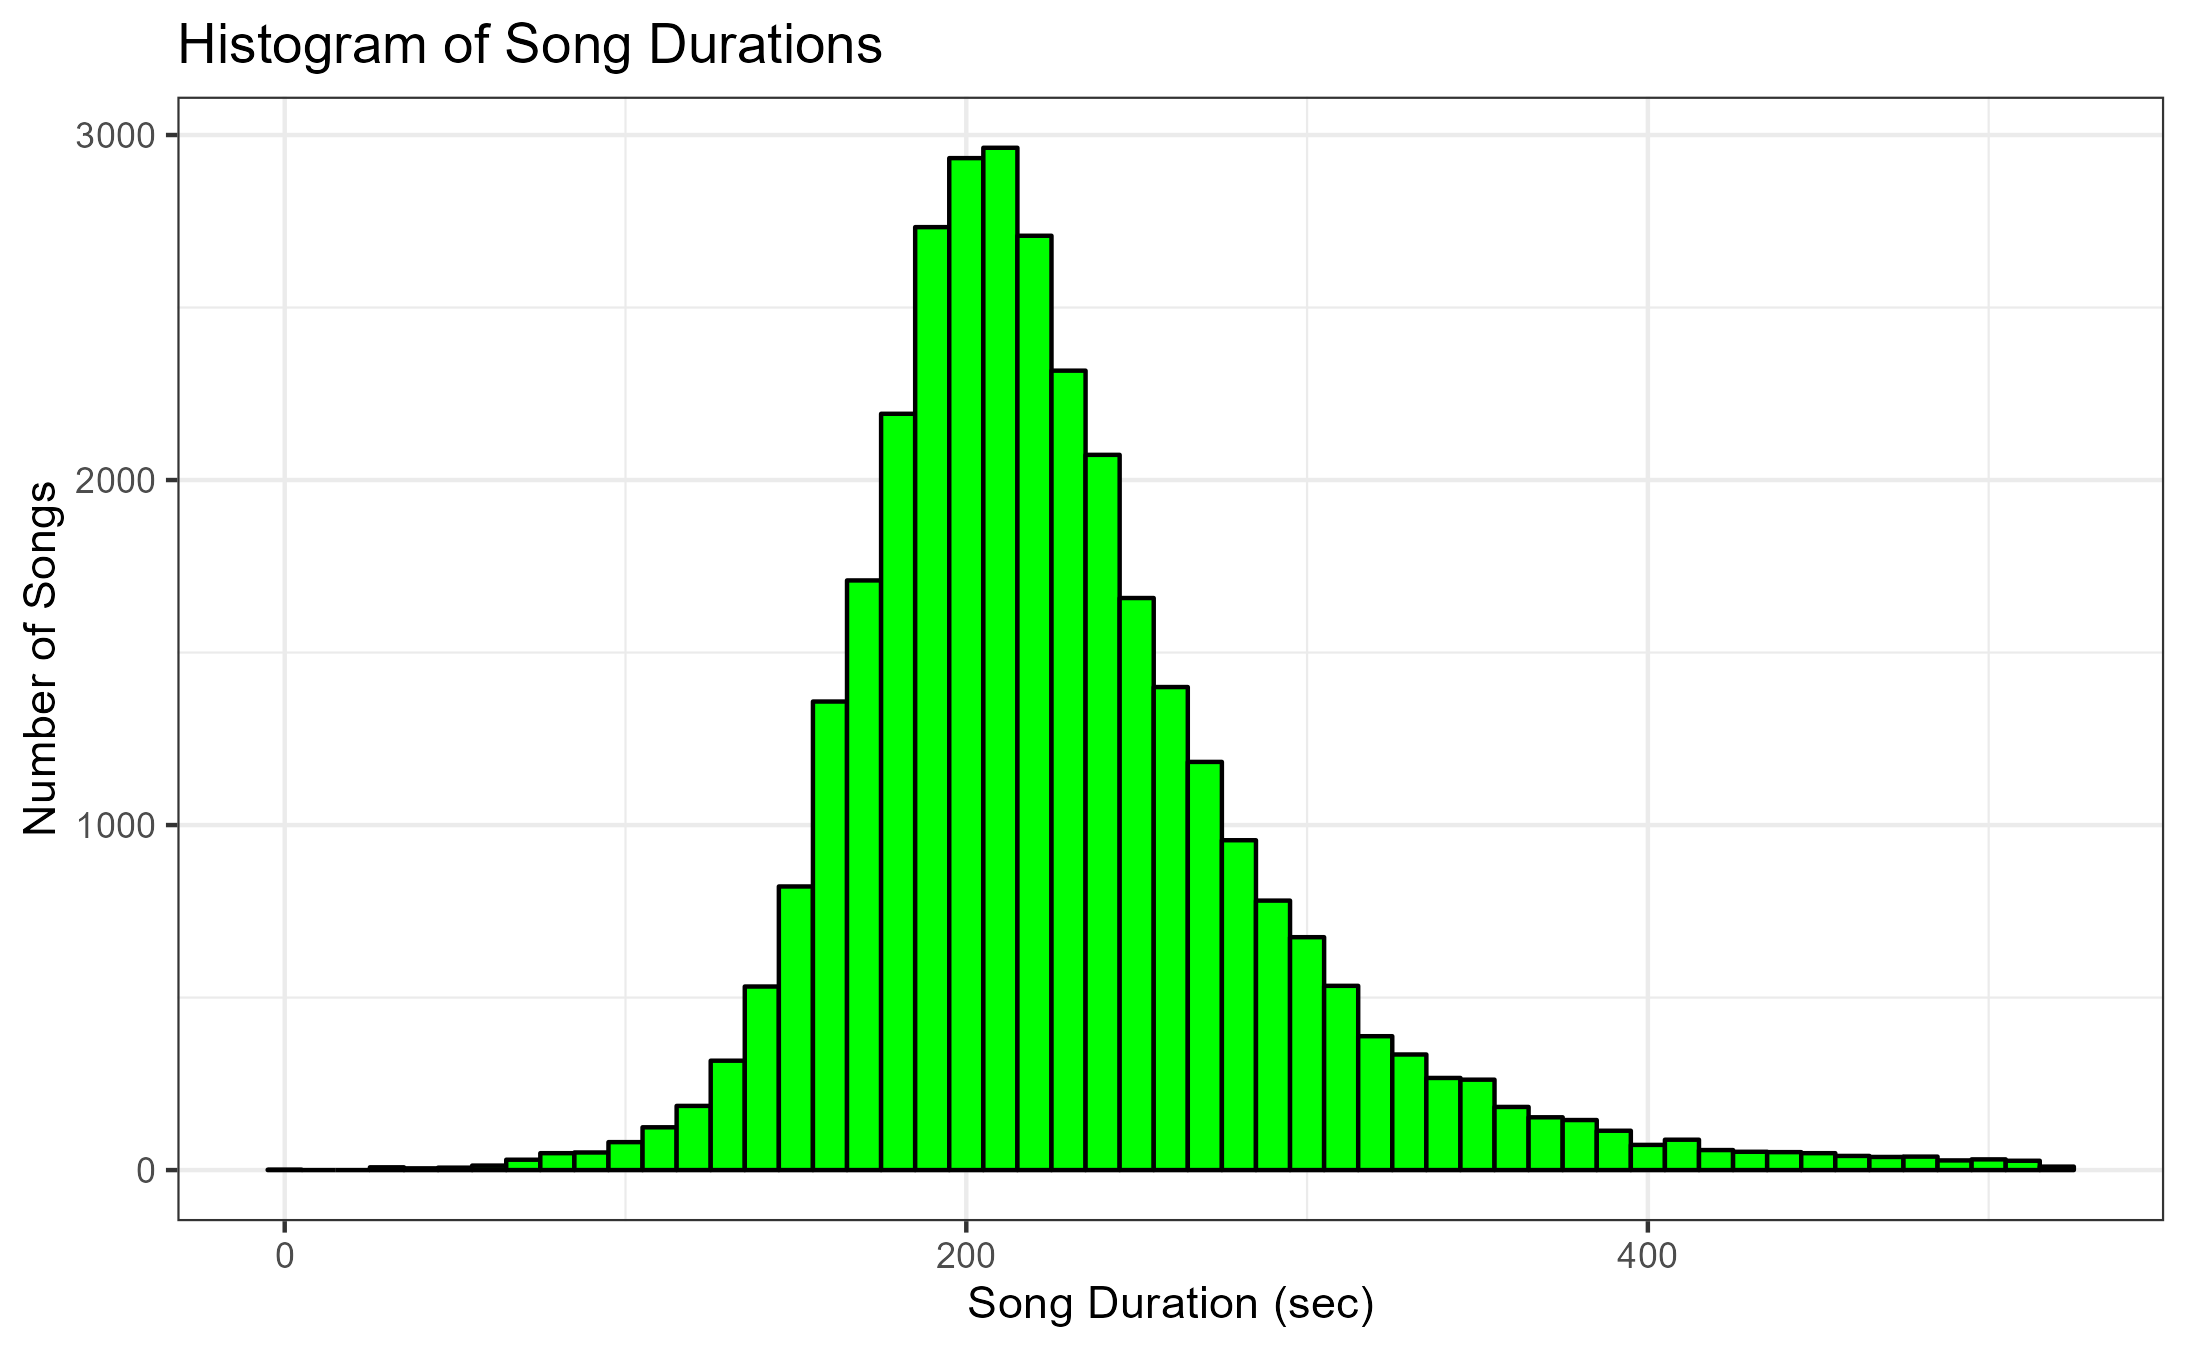
\includegraphics[scale=0.9]{slike/Histogram of song durations.png}
        %veličina slike u odnosu na originalnu datoteku i pozicija slike
        \centering
        \caption{Histogram of song duration}
        
    \end{figure}


\eject




	\chapter{Zaključak}

Kroz ovu eksploratornu analizu obradili smo mnogo stvari, od zanimljivih vizualizacija do jednostavnih prediktivnih modela. Proučili smo razne ovisnosti varijabli pjesama, žanrova i slično.
	
Vidjeli smo kako u prosjeku Trevor Daniel ima najpopularnije pjesme, 2019. je prosječna popularnost pjesama bila najviša, pop i latin imaju najpopularniju glazbu, vidjeli smo približno normalnu razdiobu trajanja pjesama i još mnogo toga.

 Stvorili smo linearni model za predikciju energije pjesama te klasifikacijski model za predikciju žanrova pjesama. Uočili smo kako se energija može dosta dobro predvidjeti kroz ostale ulazne varijable, dok za žanrove ipak postoji više grešaka u predikcijama. Okvirno model radi dosta dobro.

\eject






\end{document}
